\begin{figure}[th]
    \centering
    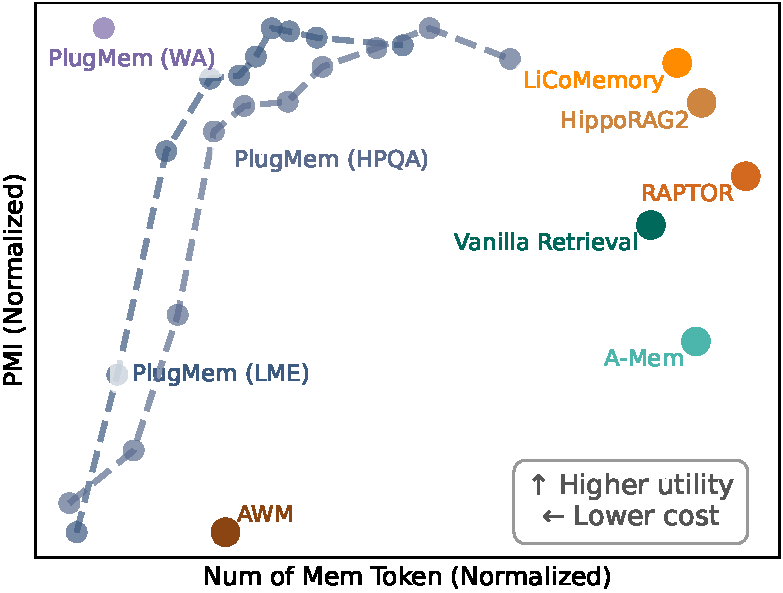
\includegraphics[width=0.4\textwidth]{Figures/hero_figure.pdf} 
    \caption{\label{fig:hero_figure}
    A utility–cost visualization of agentic memory approaches.\footnotemark \textbf{\mbox{\plugmem}, evaluated unchanged across heterogeneous benchmarks requiring processing multiple memory types, achieves the highest decision-making utility of memory at the lowest agent-side memory cost.}
    }
\end{figure}

\footnotetext{Each point corresponds to a memory method evaluated on at least one of three benchmarks, i.e., LongMemEval~\citep{wu2024longmemeval}, HotpotQA~\citep{yang2018hotpotqadatasetdiverseexplainable} and WebArena~\citep{zhou2024webarenarealisticwebenvironment}, plotted in a normalized utility–cost space to enable cross-task visualization and to accommodate baselines that are not applicable to all benchmarks. Both axes are min–max normalized, which linearly rescales values to a fixed range (e.g., $[0,1]$) while preserving relative ordering across methods. Curves are obtained by sweeping the memory token budget. The normalization is applied solely for visualization; detailed benchmark-specific analyses using raw PMI values and token numbers are reported in Section~\ref{sec:experiments} and Figure~\ref{fig:utility_cost}.}

